\documentclass[12pt, a4paper]{article}

\usepackage[utf8]{inputenc}
\usepackage{graphicx}
\usepackage{amsmath}
\usepackage{hyperref}
\usepackage{booktabs}
\usepackage{geometry}
\usepackage{setspace}
\usepackage{caption}
\usepackage{subcaption}
\usepackage{float}
\usepackage{authblk}
\usepackage{cleveref}

\geometry{margin=1in}
\setstretch{1.5}

\title{\textbf{Deep Learning Model for HIV-1 Subtype Classification Using the \textit{pol} Gene}}
\author{Jovita Nagawa}
\affil{MSB7216: Deep Learning for Health Data — Final Project Report}
\date{May 2026}

\begin{document}

\maketitle

\vspace{1cm}
\tableofcontents

\newpage

\begin{abstract}
\noindent HIV-1 genetic diversity impacts disease progression and drug resistance. Accurate subtype classification is crucial, particularly where multiple subtypes co-circulate. Traditional tools require computationally expensive multiple sequence alignment (MSA). We propose an alignment-free approach using deep learning on unaligned nucleotide data from the \textit{pol} gene. Addressing severe class imbalance with Focal Loss, we benchmark an MLP, 1D-CNN, and a Bidirectional LSTM (BiLSTM). Using 5,564 LANL sequences, our BiLSTM successfully captures long-range dependencies, achieving 94.73\% accuracy. In contrast, local spatial motifs failed, with the CNN collapsing to 52.22\%. The BiLSTM model is deployed via a Gradio web application with Monte Carlo Dropout for uncertainty estimation.
\end{abstract}

\section{Introduction \& Related Work}
HIV-1 exhibits high genetic variability, with subtypes showing distinct geographic clustering and clinical outcomes \cite{solis2018open}. Subtype identification is critical for predicting antiretroviral efficacy, designing vaccines, and epidemiological surveillance \cite{fabris2019deep}. Traditional subtyping relies on MSA, an $O(n^2)$ bottleneck \cite{pineda2013automated, struck2014comet}. K-mer methods avoid alignment but discard positional information \cite{solis2018open}. Deep learning offers an alternative by learning features directly from raw data \cite{lecun2015deep}. While CNNs excel at detecting local motifs \cite{alipanahi2015predicting}, Recurrent Neural Networks (RNNs) capture long-range dependencies. We strip alignment gaps and encode raw nucleotides, enabling the network to learn complex motifs organically without MSA, differentiating our approach from traditional tools and foundation models like DNABERT \cite{ji2021dnabert}.

\section{Dataset Characteristics}
\subsection{Data Acquisition and Filtering}
We obtained 9,264 \textit{pol} coding sequences from the LANL HIV Database \cite{lanldatabase}. After filtering for pure subtypes (A, B, C, D), removing sequences with $>5\%$ ambiguity, and deduplicating, we retained 5,564 sequences. These were split 70/15/15 (Train/Val/Test) with strict stratification.

As \Cref{fig:subtype_dist} shows, the data exhibits severe class imbalance (Subtype B: 52.3\%, C: 41.4\%, A: 5.0\%, D: 1.3\%).

\begin{figure}[H]
    \centering
    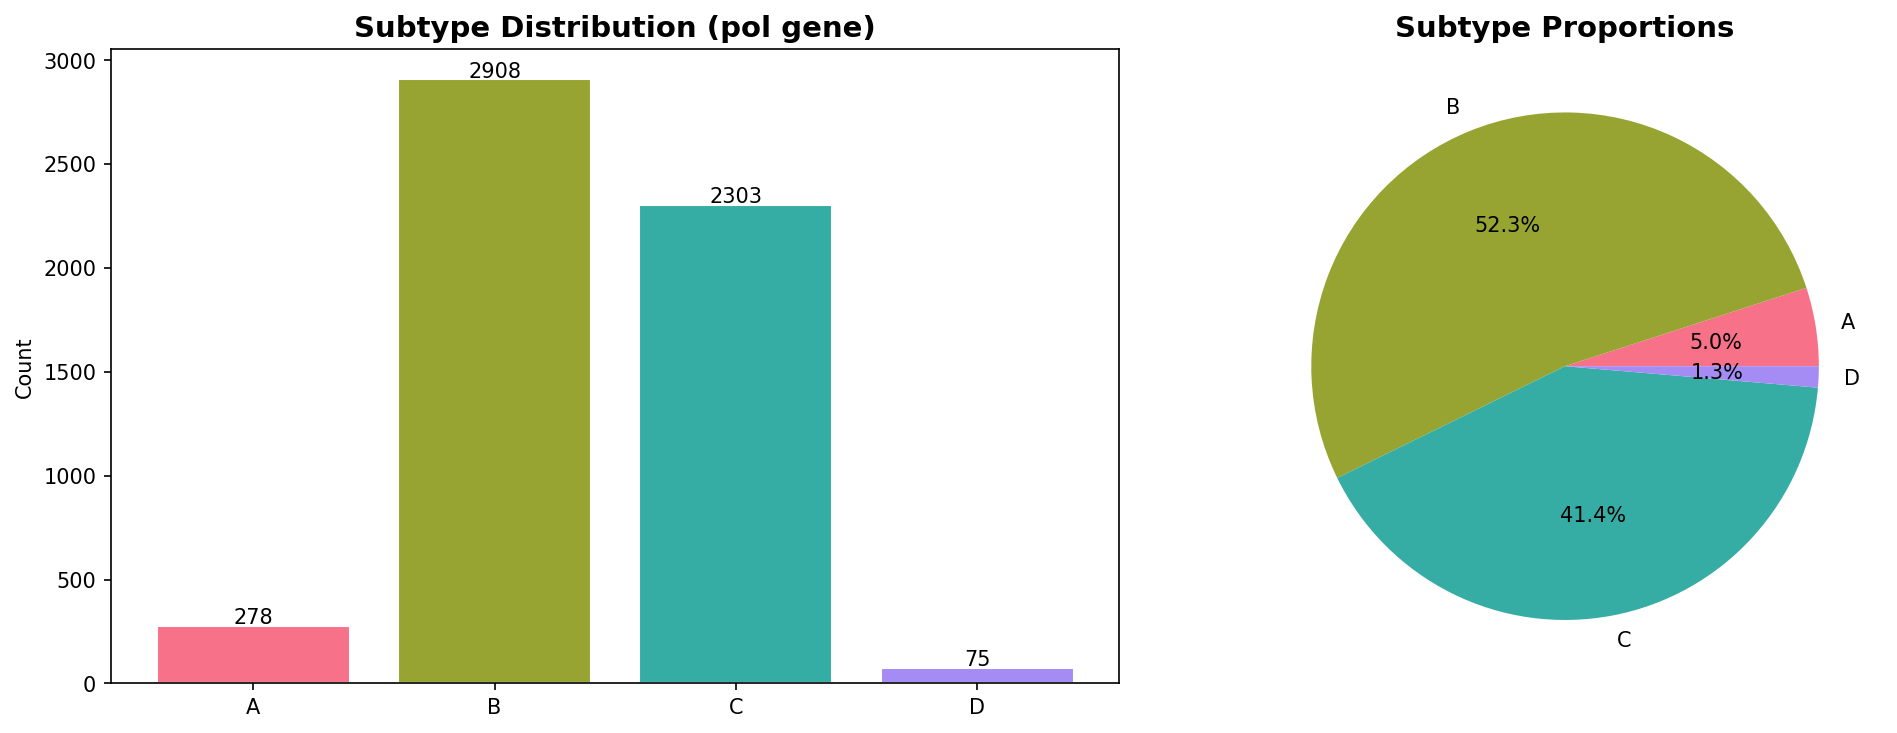
\includegraphics[width=0.85\textwidth]{figures/subtype_distribution.png}
    \caption{Severe class imbalance skewed toward Subtype B.}
    \label{fig:subtype_dist}
\end{figure}

\begin{figure}[H]
    \centering
    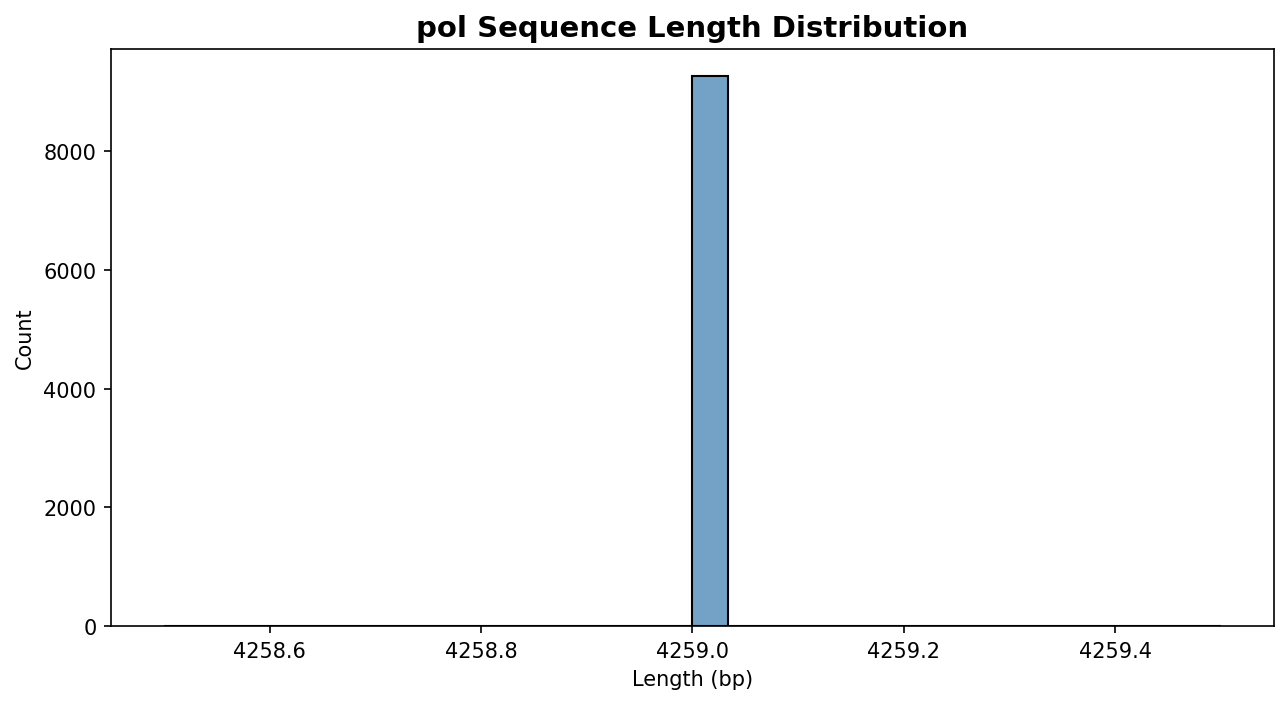
\includegraphics[width=0.85\textwidth]{figures/original_sequence_lengths.png}
    \caption{Original lengths (4,259 bp with gaps).}
    \label{fig:original_seq_lengths}
\end{figure}

\begin{figure}[H]
    \centering
    
\includegraphics[width=0.85\textwidth]{figures/sequence_lengths.png}
    \caption{Gap-stripped lengths vary significantly (2,500-4,200 bp).}
    \label{fig:seq_lengths}
\end{figure}

Contrasting \Cref{fig:original_seq_lengths} with \Cref{fig:seq_lengths} reveals that gap-stripping exposes high natural length variability, requiring dynamic padding.

\section{Methodology}
\subsection{Encoding and Class Imbalance}
We strip gaps to enforce alignment independence. Nucleotides are one-hot encoded into 4-dimensional vectors; ambiguous bases become zero vectors. A custom collate function dynamically zero-pads batches to the longest sequence, optimizing memory. To counter class imbalance, we utilize Focal Loss \cite{lin2017focal} ($\gamma=2.0$) with inverse-frequency weights, penalizing easy majority examples and focusing on minority classes like Subtype D.

\subsection{Model Architectures}
We compared three architectures:
\begin{enumerate}
    \item \textbf{MLP (Baseline)}: Adaptive pooling to 64 positions followed by dense layers. Destroys motif structures.
    \item \textbf{1D-CNN}: Four convolutional blocks (kernel sizes 7, 5, 3) followed by global adaptive pooling, designed to capture local motifs.
    \item \textbf{BiLSTM}: Embeds nucleotides to 128-d, processes via a 256-d BiLSTM to capture global contextual dependencies across the entire sequence.
\end{enumerate}

\section{Experiments and Training}
Models were trained with AdamW and Cosine Annealing on a Colab T4 GPU. The CNN converged rapidly to 97.74\% training accuracy by epoch 2 but collapsed on validation. The BiLSTM required 12 epochs to reach optimal validation loss, showing stable learning compared to the highly volatile MLP baseline.

\begin{figure}[H]
    \centering
    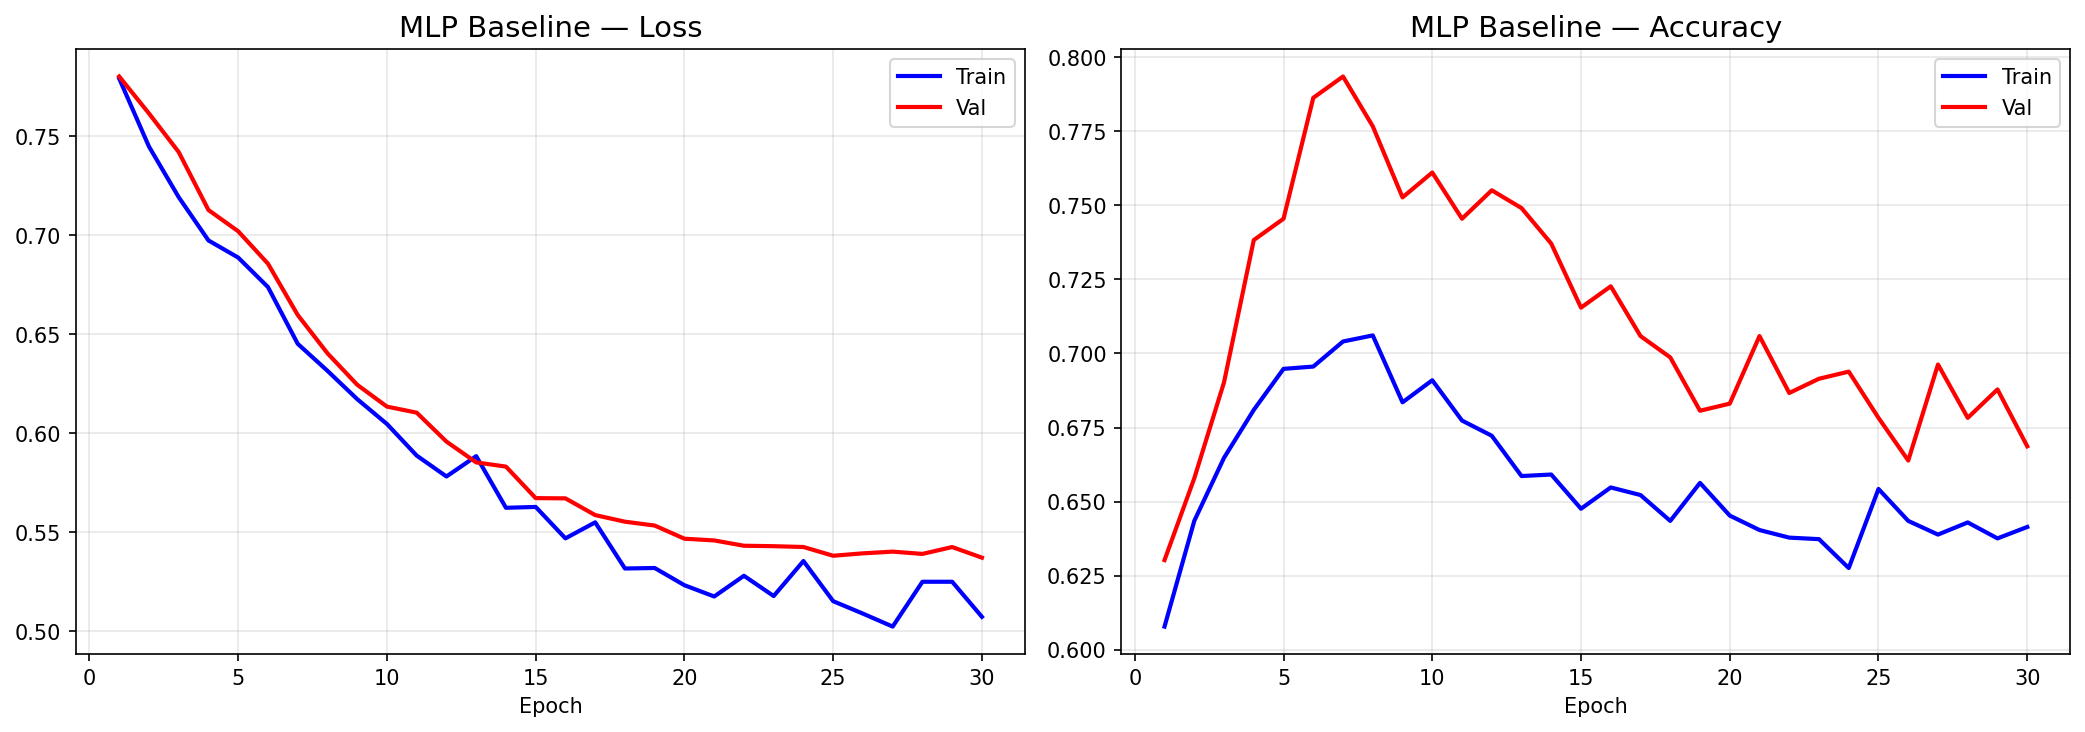
\includegraphics[width=0.85\textwidth]{figures/baseline_mlp_training_curves.png}
    \caption{Baseline MLP volatility.}
\end{figure}

\begin{figure}[H]
    \centering
    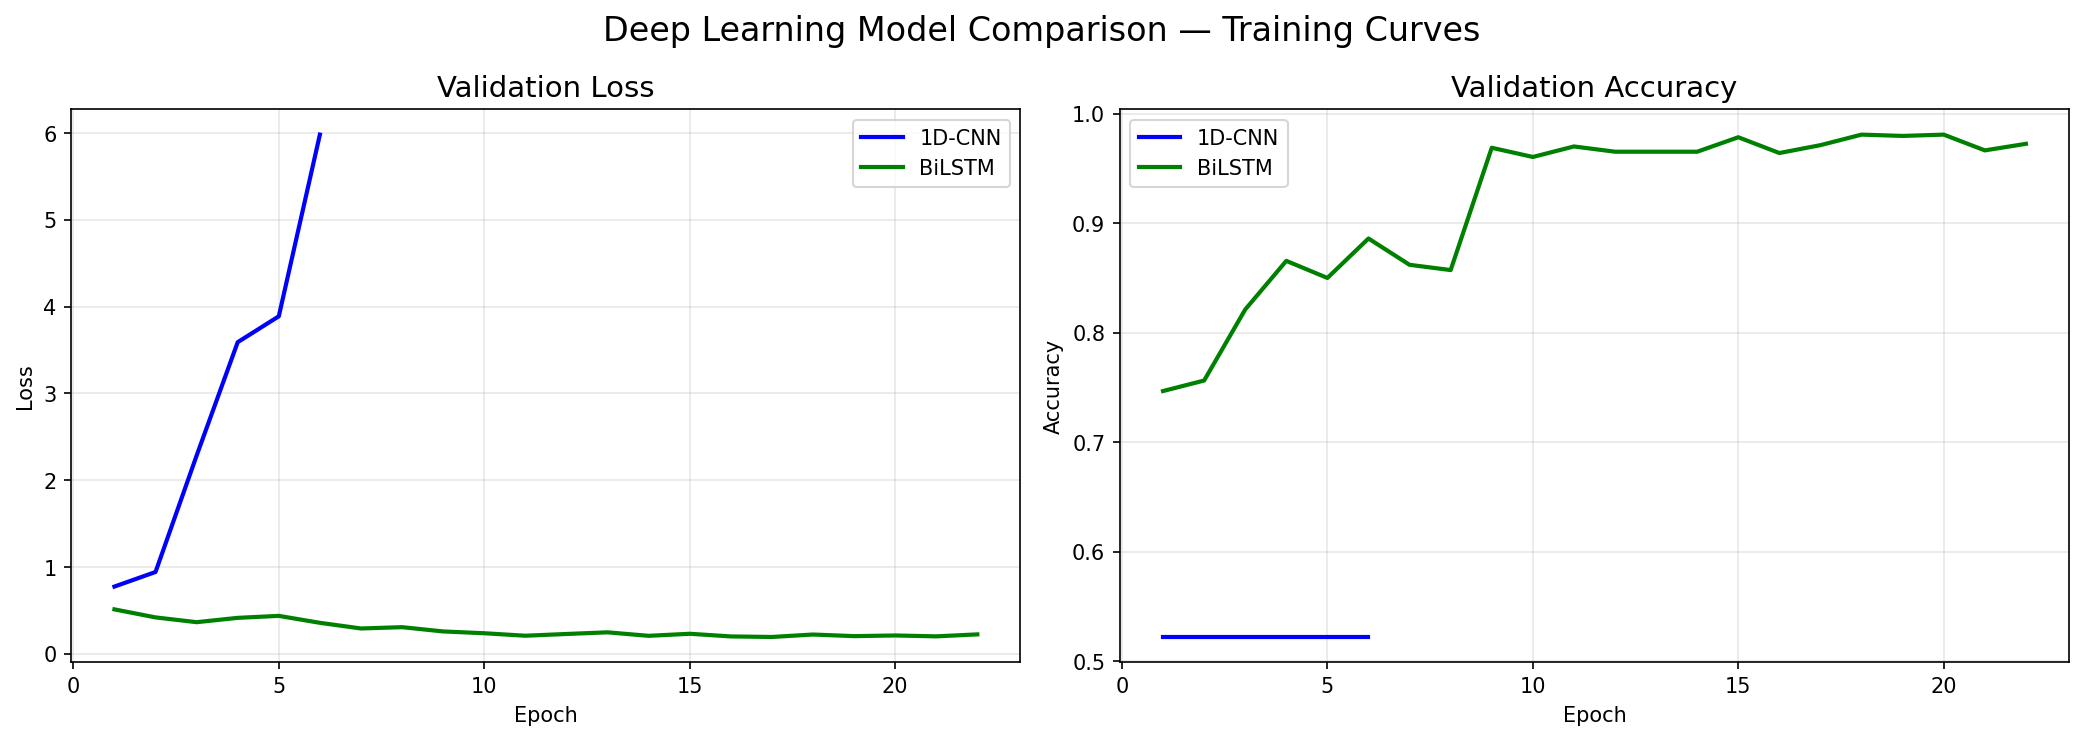
\includegraphics[width=0.85\textwidth]{figures/model_comparison_curves.png}
    \caption{Model Comparisons.}
    \label{fig:training_curves}
\end{figure}

\section{Results and Discussion}
The BiLSTM significantly outperformed all models (\Cref{tab:results}), proving subtype discrimination requires global bidirectional dependencies. The CNN collapsed entirely to the majority class (52.22\%), exposing the insufficiency of local motifs for unaligned sequences.

\begin{table}[H]
    \centering
    \begin{tabular}{lcccc}
    \toprule
    \textbf{Model} & \textbf{Accuracy} & \textbf{Macro F1} & \textbf{Precision} & \textbf{Recall} \\
    \midrule
    \textbf{BiLSTM} & \textbf{94.73\%} & \textbf{0.6541} & \textbf{0.6274} & \textbf{0.6982} \\
    MLP Baseline & 65.27\% & 0.5114 & 0.5082 & 0.7472 \\
    1D-CNN & 52.22\% & 0.1715 & 0.1305 & 0.2500 \\
    \bottomrule
    \end{tabular}
    \caption{Test Set Performance.}
    \label{tab:results}
\end{table}

\begin{figure}[H]
    \centering
    
\includegraphics[width=0.85\textwidth]{figures/best_model_roc.png}
    \caption{BiLSTM ROC Curves.}
    \label{fig:roc}
\end{figure}

\begin{figure}[H]
    \centering
    
\includegraphics[width=0.85\textwidth]{figures/best_model_per_class_metrics.png}
    \caption{BiLSTM Per-class metrics.}
    \label{fig:per_class}
\end{figure}

\begin{figure}[H]
    \centering
    
\includegraphics[width=0.9\textwidth]{figures/all_confusion_matrices.png}
    \caption{Confusion Matrices across models.}
    \label{fig:confusion}
\end{figure}

The BiLSTM misclassified only 44/835 sequences (5.3\% error). However, it failed entirely on Subtype D (0\% recall) due to extreme data starvation (only 53 training instances). Most misclassifications (e.g., B predicted as A) occurred with high confidence (mean: 0.787), biologically suggesting overlapping sequence motifs or potential recombinant forms.

\section{Conclusion and Future Work}
Deep learning effectively subtyped raw HIV-1 sequences with 94.73\% accuracy, eliminating the MSA bottleneck. The success of the BiLSTM underscores the necessity of long-range sequence context. 

Building on these findings, our immediate future work will focus on the following core objectives:
\begin{itemize}
    \item \textbf{Resample data} to effectively balance the minority classes (especially Subtype D) and retrain the model to prevent collapse.
    \item \textbf{Finetune the CNN} to check for any possible better performance, specifically investigating if optimized hyperparameters or alternative pooling mechanisms can overcome its current spatial limitations.
    \item \textbf{Expand} the classification scope to include Circulating Recombinant Forms (CRFs) and other complex subtypes, ensuring the tool reflects the true diversity of the global epidemic.
\end{itemize}

The codebase and an uncertainty-aware deployment application are available open-source (\url{https://github.com/jnagawa/hiv-subtype-classifier}).

\bibliographystyle{plain}
\bibliography{references}
\end{document}
